%%%%%%%%%%%%%%%%%%%%%%%%%%%%%%%%%%%%%%%%%%%%%%%%%%%%%%%%%%%%%%%%%%%%%%
% LaTeX Example: Project Report
%
% Source: http://www.howtotex.com
%
% Feel free to distribute this example, but please keep the referral
% to howtotex.com
% Date: March 2011 
% 
%%%%%%%%%%%%%%%%%%%%%%%%%%%%%%%%%%%%%%%%%%%%%%%%%%%%%%%%%%%%%%%%%%%%%%
% How to use writeLaTeX: 
%
% You edit the source code here on the left, and the preview on the
% right shows you the result within a few seconds.
%
% Bookmark this page and share the URL with your co-authors. They can
% edit at the same time!
%
% You can upload figures, bibliographies, custom classes and
% styles using the files menu.
%
% If you're new to LaTeX, the wikibook is a great place to start:
% http://en.wikibooks.org/wiki/LaTeX
%
%%%%%%%%%%%%%%%%%%%%%%%%%%%%%%%%%%%%%%%%%%%%%%%%%%%%%%%%%%%%%%%%%%%%%%
% Edit the title below to update the display in My Documents
%\title{Project Report}
%
%%% Preamble
\documentclass[paper=a4, fontsize=11pt]{scrartcl}
\usepackage[T1]{fontenc}
\usepackage{fourier}

\usepackage[english]{babel}															% English language/hyphenation
\usepackage[protrusion=true,expansion=true]{microtype}	
\usepackage{amsmath,amsfonts,amsthm} % Math packages
\usepackage[pdftex]{graphicx}	
\usepackage{url}


%%% Custom sectioning
\usepackage{sectsty}
\allsectionsfont{\centering \normalfont\scshape}


%%% Custom headers/footers (fancyhdr package)
\usepackage{fancyhdr}
\pagestyle{fancyplain}
\fancyhead{}											% No page header
\fancyfoot[L]{}											% Empty 
\fancyfoot[C]{}											% Empty
\fancyfoot[R]{\thepage}									% Pagenumbering
\renewcommand{\headrulewidth}{0pt}			% Remove header underlines
\renewcommand{\footrulewidth}{0pt}				% Remove footer underlines
\setlength{\headheight}{13.6pt}


%%% Equation and float numbering
\numberwithin{equation}{section}		% Equationnumbering: section.eq#
\numberwithin{figure}{section}			% Figurenumbering: section.fig#
\numberwithin{table}{section}				% Tablenumbering: section.tab#


%%% Maketitle metadata
\newcommand{\horrule}[1]{\rule{\linewidth}{#1}} 	% Horizontal rule

\title{
		%\vspace{-1in} 	
		\usefont{OT1}{bch}{b}{n}
		%\normalfont \normalsize \textsc{} \\ [25pt]
		\horrule{0.5pt} \\[0.4cm]
		\normalsize Interactive Theorem Proving - A. Chlipala (Notes) \\
		\horrule{2pt} \\[0.5cm]
}
\author{
		\normalfont 								\normalsize
        Satyendra Kumar Banjare\\[-3pt]		\normalsize
        \today
}
\date{}

\begin{document}
\maketitle
\section{Lecture 1}
This is a fair introduction to what is the basic idea of interactive theorem proving. We are given some pre conditions 	, post conditions and the core idea/theorem to check. Examples include :
\begin{itemize}
	\item{
		Solving a  simple linear equation for x, eg: $ y = m*x +b $ . The pre conditions are that $m \neq 0 $. Post conditions involve the value of x obtained actually satisfies the original equation. 
	}
	\item{Alias analysis involves determination of optimum strategy to find the number of ways a particular memory address can be accessed. using ITP techniques we can assertain this by checking and case elimination of redundant pointers. 
	}

	\item{Anderson's Analysis}
Often called Anderson-Style Pointer analysis involves the flow sensitive pointer analysis and pointer mutation. It follows assigning a set-notation to pointers bounded by given constraints. It treats all allocations done by one instruction as if they are being done to only 1 object. We define $PT(x)$ as a set that approximats all the locations that can be ppointed by the variable x. Different constraints are generated according to the type of modifications done. We then case-by-case analize them. for better examples : \url{https://www.seas.harvard.edu/courses/cs252/2011sp/slides/Lec06-PointerAnalysis.pdf}. 

\end{itemize}

\section{Lecture 2}
The lecture 2 introduces the idea of first order logic, propositional logic and the deduction system. The proofs are merely a set of ad-hoc ideas that use high level argument techniques to finally achieve the assumed equational equivalence. An example of proving by induction is explained in the lecture. We should be able to reason every step we take to achieve our next small goal. 

\begin{itemize}
	\item{ \textbf{Propositional Logic} is like SAT problem or rather we should say that SAT problem is an example of propositional logic. The variables used are assumed boolean and equations formed from them are assumed to be a deductive property. The outcome is desired only if the initial conditions are met. Hence the deduction system is defined and is expressed as :

	\[ \dfrac{A \; B}{ A \: \Lambda \: B } \rightarrow I \]

	for a derived property I.

	Natural Deduction uses base coditions as some inital properties that may themselves be derived from some other.
	}

	\item{ \textbf{First Order Logic} can be understood as a general mathematical statement made that may or may not have a constraint domain and range. A infinite possible cases may be generalized and hence 'Truth Table' analogue is diffficult to produce. In this case thus we can use Natural Deduction techniques to develop a more concrete system to analize things. 

	}
\end{itemize}

\section{Lecture 3}
The Lecture 3 introduces the idea of Peano's Axioms and contradicts the set theory approach and argues the approach of using some inductive defiitions and basic data structure to be the more fundamental foundational mathematics theory - the basic idea of Type Theory. The Coq Proof system is also dependent on Type theory fundamentals and has some very basic data structure ideas and possibility of recursive definitions.In Coq Terminology, Inductive Definitions and Fixpoint Definitions (for recursive definitions) are defined to get the readers an idea of doing theing using type theory fundamentals. Proof state Reductions are also explained with a small example. Coq Tactic  : Reflexivity is also introduced. 

\section{Lecture 4}
This Leture explains proving some basic and important properties like transitivity for a 'LessThan' definition using Coq theorem prover. We learnt to use inductive hypotheses to achieve goals and prove theorems. At one point we also learnt the key pint differences in a Fixpint nad Inductively defined definitiins of some or the other property. 

The Later Examples include :

\begin{itemize}
	\item{ \textbf{Turing Machines} in theory requires state transitions to complete a given process. This transitions are often unique and the states may be related to more than one process. Thus easily forming a given state and then using an arbitrary trnasition we may reach expected final state without having to think how we reached the first state initially. This may be expressed in the form of deductive hypotheses and first order logic as explained in the example.
	} 
	\item{\textbf{List Sorting} can be understood and often proved using induction, saying if a list is sorted then every part of it is also sorted.
	}
	\item{\textbf{Programming Language Interpreter} was the best possible example explained here where a context free grammar for a given language was written in a form that can be easily represented in the proof system.
	}
\end{itemize}

\section{Lecture 6}
This is an introduction to Coq tactical techniques for easy proving things by reducing proof states by using computational equivalent of then required proof terms. A simple example on type safety was explained along with development of a type system using deductive rules. We leant how the goals are sequenced both uniformly and non-uniformy (exaplained using a less than or equal to property) and introduced ourselves to the tactics \textbf{split, try}  and \textbf{repeat}. we also learnt using idtac in coq proof system.

\section{Lecture 7}
This Lecture introduces to more concrete ideas and problems on which the program verification system is built. Starting from classical program verification techniques that involved a verification generator and verification condition to new and advanced Interactive provers. There are broadly two problems stated that are faced while developing a proof system :

\begin{itemize}
	\item{Error Diagnosis and internal verification during evolution of proof states.}
	\item{Efficient design of software system.}
\end{itemize}

The Internal Verification is tedious process that face major challenges like :

\begin{itemize}
	\item{\textbf{Verbosity} : Deciding the level upto which the code should be made verbose. }
	\item{\textbf{Runtime Efficiency} : The written code should be effiently run on most of host systems.} 
\end{itemize}

There are some other areas touched in this lecture which are :
\begin{itemize}
\item{ \textbf{Program Extraction} deals with removing redundant code and keeping only the assumed correct end result part of code to be finally compiled and tested further. The idea of a proof-erasing compiler has beeen discussed. This extraction further boils down to deciding and optimizing how to selection producre is implemented. For a basic understanding A propery type data is to be lost but a Set type of data is preserved.
}
\item{\textbf{Coq Type Hierachy} illustrates the top level abstract data structure program extraction is based on. On the very basic $0^{th}$ level it consists of Sets and Property type datas, as one can easily guess.
}
\item{\textbf{Secure Information Flow} The Extraction basically removes all useable information from property datas so that their modification is unit steped and easy. This easily brings out concern for having a "secure" information flow ensuring an output insn't an outcome of some internal data leak or bug. 
}
\item{\textbf{Taint Analysis} deals with checking those variables whose values can be easily changed from the user input. The input made should be checked as well so that any unexpected behaviour is not witnessed.
}
\item{\textbf{Eliminatin Restrictions} prevent producing a set while eliminating a property. All other combinations like producing set and eliminating a set, producing a property and eliminating a set and producing a prop and eliminating a set are possible


\begin{figure}[!htb]
\centering
  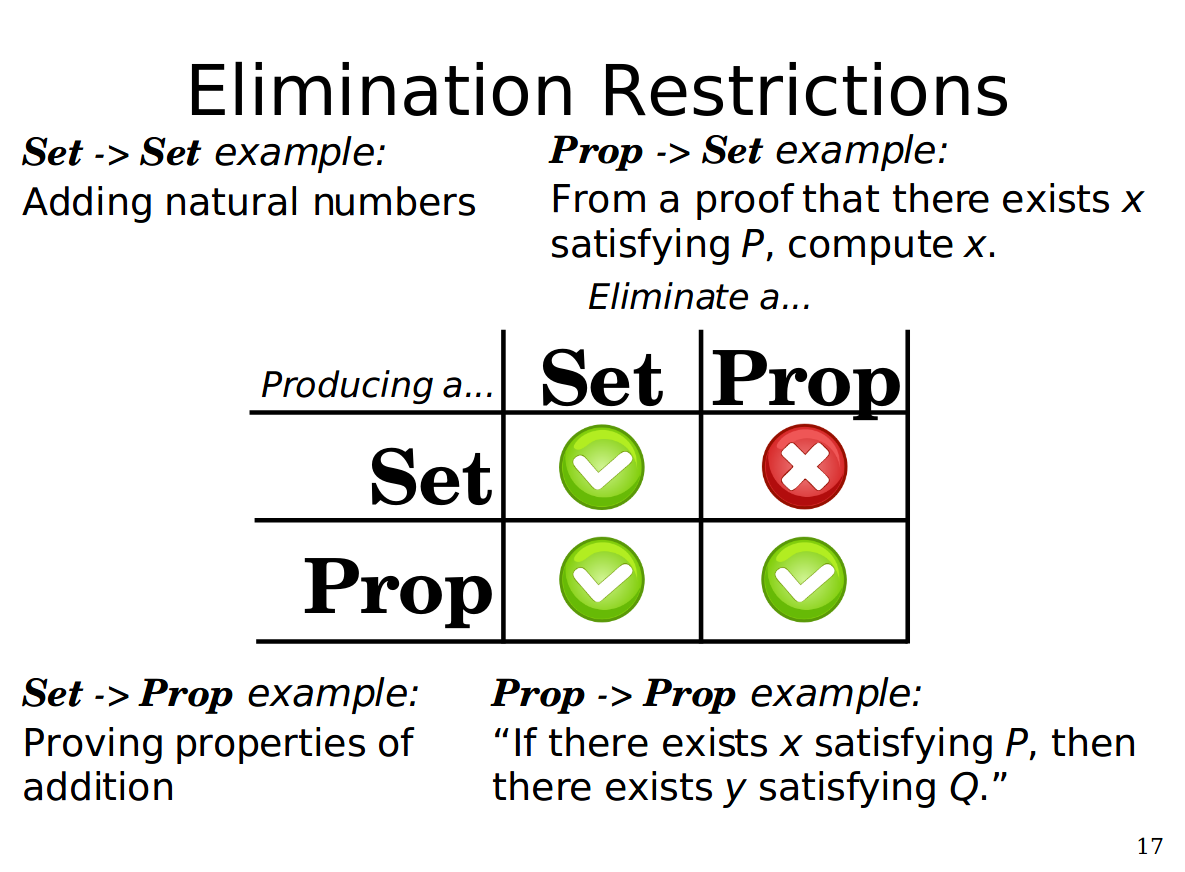
\includegraphics[width=\linewidth]{elim_restrict.png}
\end{figure}

}
\end{itemize}

\section{Lecture 9}
This lecture title "Beyond Primitive recursion" talks about recursiveness of proof states and corresponding functions starting with the importance of having a termination of a proving process. The working principle often involves using a proof A to derive a proof B. But how far this proof dependence will go on is a good question to be answered.

A well founded recursion involves those functions that do not have infinitely descending chains. The possible types of recursion include \textbf{Primitive recursion} (example : Fibonacci numbers, often defined using a fixpoint definition in Coq.), \textbf{Bounded recursion} (example : a bounded natural to Integer converter function), \textbf{Compositional Reasoning recursion} and an \textbf{Ad-Hoc recursion}. Our Proof system should always allow for a general recursion to occur to make it Turing Complete. How to achieve this ?

Well professor answers using a principled version of bounded recursion. 

\section{Lecture 11}
Having firstly solved software foundations, I was quite aware of things mentioned in this part which included the techniques refered as reflection technique for proving if a property P holds. The Tauto tactic and declaring and proving soundness (cases like :Forall numbers n) of a given property P.

It reflection technique includes making decision procedure for checking P and it returns booleans. Proving that P holds whenever that decision is true and proving the proof terms of original theorem ab using "reflexivity"  tactic.

The tauto tactic (which is also used by intuition) solves this goal by expanding out all 2n cases arising from the disjunctions in the assumption, leading to exponentially-sized proofs.

Later part of the lecture discusses using syntactic representation which includes having an Inductive definitions, for a generic decision procedure and using that to prove goals further. 

\end{document}

